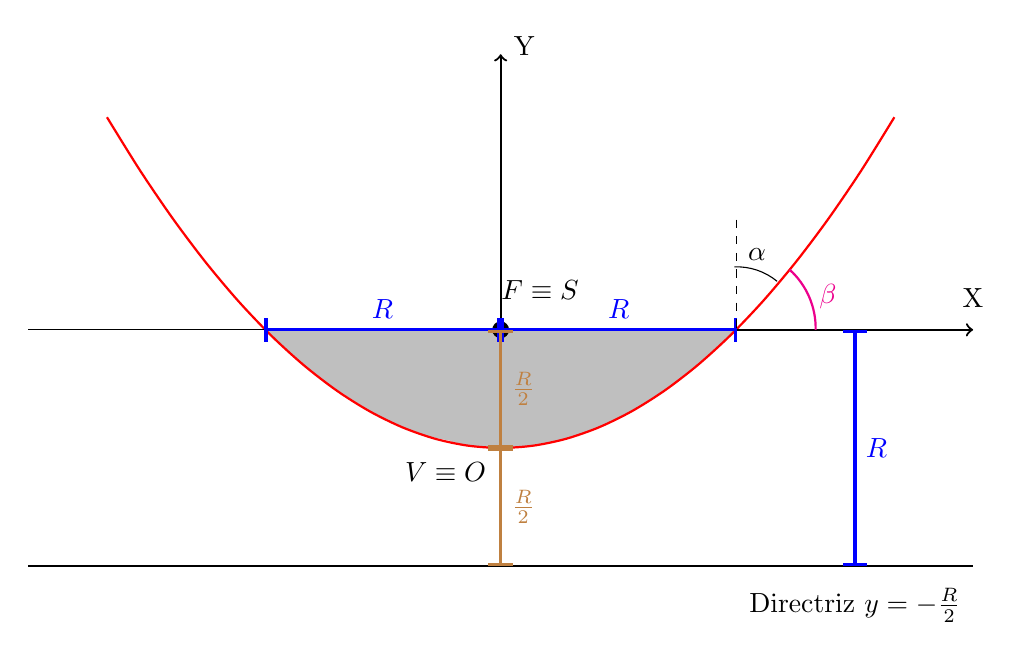
\begin{tikzpicture}
\draw  [fill, lightgray]plot[smooth, tension=0] coordinates {(-0.6255,0.0841) (-0.4436,0.0413) (-0.1975,0.0199) (0.2626,0.0199) (0.5837,0.0734) (0.8833,0.1376) (1.1508,0.2339) (1.5146,0.3837) (1.8464,0.5763) (2.2637,0.8653) (3,1.5) (2.5633,1.4966) (2.2958,1.4966) (-3,1.5) (-2.6159,1.1649) (-2.2414,0.8546) (-1.5993,0.4372) (-1.2034,0.2553) (-0.8931,0.1483) (-0.6255,0.0948)};

\draw[thick, scale=0.5,domain=-10:10,smooth,variable=\x,red] plot (\x,{0.084*\x*\x});
\draw [thick, <->](0,5) -- (0,1.5) -- (6,1.5);
\draw (-6,-1.5) -- (6,-1.5);
\draw (-6,1.5) -- (6,1.5);
\draw [fill] (0,1.5) node (v1) {} circle (0.1);
\draw [very thick, blue,|-|](-3,1.5) node (v3) {} -- (v1.center) node[midway, above]{$R$};
\draw [very thick, blue,|-|](v1.center) -- (3,1.5)node[midway, above]{$R$};
\draw [very thick, brown,|-|](0,1.5) -- (0,0)node[midway, right]{$\frac{R}{2}$};
\draw [very thick, brown,|-|](0,-1.5) -- (0,0)node[midway, right]{$\frac{R}{2}$};
\draw [very thick, blue,|-|](4.5,1.5) -- (4.5,-1.5)node[midway, right]{$R$};

\node at (4.5,-2) {Directriz $y=-\frac{R}{2}$};
\node at (-0.7,-0.3) {$V\equiv O$};
\node at (0.5,2) {$F\equiv S$};
\draw [thick, magenta](4,1.5) arc (-1.1975:48:1)node[midway, right]{$\beta$};
\draw [dashed](3,2.9) -- (3,1.5) node (v2) {};
\draw (3.5099,2.1164) arc (50.4017:92.4:0.8)node[midway, above]{$\alpha$};
\node at (6,1.9) {X};
\node at (0.3,5.1) {Y};
\end{tikzpicture}